\chapter{Flexibility}
\label{chap:Flexibility}

\funnyquote{You must be shapeless, formless, like water. When you pour water in a
cup, it becomes the cup. When you pour water in a bottle, it becomes the
bottle. When you pour water in a teapot, it becomes the teapot. Water can drip
and it can crash. Become like water my friend.}
{Bruce Lee}

Any system exhibits particular compromises between opposing goals. Some
constraints derive from the nature of the problem a particular system is trying
to solve. Different problems might have conflicting constraints. It follows
that to assert the flexibility of a system, we need to choose particular use
cases and leave out others. This chapter presents the uses cases we chose to
support and how they can be implemented using our design.

%TODO: Explain that for most examples, we will directly use the implementation
%      language, while it could also have been possible to expose some primitive
%      operations to the source language

We will see different examples modifying the base system to adapt it to
particular use cases. The examples are written either in the implementation
language of the VM, which has a direct access to the object representation and
the execution environment or in the source language, which does not and
correspond to the execution environment of user-supplied code. In other words,
the implementation language is executed directly on the host VM and the source
language is first translated to execute in a virtualized environment like
regular source code. A comment line at the beginning of each example explicitly
states if the example is written in the implementation language or the source
language.

We first explore how to obtain object model operation information by redefining
their corresponding methods.  We then see how to obtain a dynamic call graph by
redefining the \kw{call} method on functions. Both of these support our thesis,
by showing how the object model and the function calling protocol can be
instrumented. Finally, we discuss ways to enforce runtime invariants used to
catch common programming mistakes to show that although our focus was on
building instrumentation infrastructure, the resulting system has broader
applicability than the context in which it was developed.

\section{Obtaining object model operation information}
\label{sec:ObjectModelInstrumentation}

Given a good approximation of the performance cost of JS operations, such as
property accesses and object creation, we might be interested in estimating the
performance of an application by computing the number of run-time occurrences of
each of these operations.

The design of the system makes it easy to do this by wrapping the method
implementing the semantic operation with a function incrementing a counter.  In
the following example, we do it for property accesses, property assignments
and property deletions. The following example shows an example of
instrumentation code for the object model, expressed in the
implementation language:

\jsfile{listings/object-model-instrumentation.js}

This instrumentation can be exercised with the following example, written in
the source language:

\jsfile{listings/object-model-instrumentation-test.js}

It should give a count of one for property assignments, a count of two for
property accesses and a count of three for property deletions.

Notice that the instrumentation is granular in time, namely it can be activated
and interrupted at any moment.  To cover the entire application execution,
instrumentation need simply be activated before an application is actually
started. 

\section{Obtaining a dynamic call graph}

A dynamic call graph is a data structure encoding the calling relationship
between functions, occurring during the execution of a program. For example, if
a function \kw{a} calls a function \kw{b}, the \textit{a calls b} relationship
will be registered in some way. 

Dynamic call graphs can be used to determine the code coverage of unit tests as
well as to provide detailed runtime information for code comprehension,
run-time optimizations and analyses of source code. 

Context-insensitive call graphs do not encode the calling context of a call,
while context-sensitive call graphs do. For context-insensitive call graphs, we
might represent functions as nodes and calling relationships as edges.
Context-sensitive call graphs could represent functions as multiple nodes,
depending on their respective callers. For the sake of simplicity, we will
consider a context-insensitive call graph for the remainder of this example. 

As seen previously in the design chapter~(\ref{chap:Design}), function calls
origin from four sources in the language: global function calls, method calls,
indirect calls through \kw{call} and \kw{apply} and direct calls to functions
stored in variables. By redefining the \kw{call} and \kw{apply} methods, we can
intercept every call made from these four origins.

The following program will be traced and exhibits every case enumerated
above. Four different functions are declared and two are initially called:

\jsfile{listings/callgraphexample.js}

In this example, \kw{c} calls \kw{b}, \kw{b} calls \kw{a}, and \kw{a} calls no
other function, \kw{e} recursively calls itself but no other function and
\kw{d} is not called nor calls another function. We would expect a call graph
like the one shown in Figure~\ref{fig:CallGraph} to model those relationships.

\begin{figure}[htb]
\begin{center}
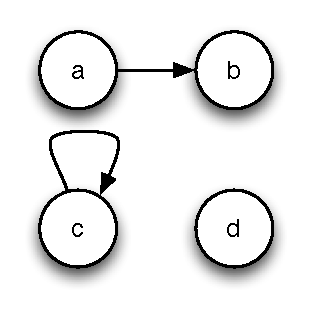
\includegraphics{figures/callgraph}
\caption{\label{fig:CallGraph} Call Graph for example code}
\end{center}
\end{figure}

A context-insensitive analysis requires a single node per function. Therefore,
we can store the profiling information directly on the functions themselves.
This way it avoids the complexity associated with maintaining separate data
structures and maintaining a correspondence between functions and those data
structures.

\subsection{Protecting the profiling code in a critical section} 

A \textit{critical section} usually refers to a section of code in a
multi-threaded program in which the system guarantees that no preemption will
occur. By analogy, we use the term to refer to a section of code in a profiled
program in which the system guarantees that no profiling occurs.

By using a critical section, we solve the issue of having the profiling code
being profiled. It is important to avoid profiling the profiling code, not only
because it pollutes results but mostly because it can introduce
\textit{meta-stability} issues, namely that performing an operation in the
profiling code might call back into the same operation being profiled, creating
an infinite loop.

A critical section can be implemented by introducing a flag that controls
whether profiling occurs or not. Just before the profiling code starts
executing, the flag is set and right after the profiling code ends the flag is
reset. It can be done with a boolean variable if the section needs not be
reentrant or with a integer otherwise.

When profiling JS function calls, we need to be cautious about the different
ways the flow of control can be manipulated by the callee. In JS, a function
can return either normally through its explicit or implicit return statement or
by raising an exception. Fortunately, JS provides a \kw{finally} construct that
guarantees that however the flow of control leaves a try block, the \kw{finally}
block will always be executed. We can therefore perform pre-call operations in
a \kw{try} block and perform post-call operations in a corresponding
\kw{finally} block.

The next requirement is to be able to intercept every function call in the
program. Our design makes it easy by reducing every occurrence of function calls
to sending the message \kw{call} or \kw{apply} to the called function, whether
it is global, local or is a method. We can further implement \kw{call} in terms
of \kw{apply}, which gives us a single point of instrumentation for the whole
system. By redefining the \kw{call} and \kw{apply} methods on the root function,
we can profile the whole system.

The only problem left with this approach comes from the circularity introduced by
having every JS object operation and function invocation performing a
\kw{call}. It means that no primitive operation in the source language can be
used to perform a call. We solve it by performing the instrumentation in the
implementation language.~\footnote{Extensions to the source language could also
have been made, in which case the source language could have been used to the
same effect.}

The next example introduces two instrumentation primitives as global functions
in the source language, \kw{startCallInstrumentation} and
\kw{stopCallInstrumentation}. When called, the instrumentation function
initializer redefines the \kw{call} and \kw{apply} methods on the root function
and uses the \kw{before} and \kw{after} source-language functions to perform
pre- and post-call operations.  By virtue of the critical section, any operation
performed by \kw{before} and \kw{after} will not be profiled:

\jsfile{listings/dyn-call-graph-instr.js}

This definition has an interesting property: the initialization of the call
instrumentation is atomic and will take effect the next time a call is
performed but will not affect any function currently in the calling context.
Likewise, the instrumentation can be changed or stopped on-the-fly but the
previous instrumentation will still performs its post-call operations on
functions currently in the calling context.

The previous listing was essentially an extension of the implementation to
allow function call instrumentation. The next listing uses that extension to
build a dynamic call graph. It registers all called functions on a shadow stack
as well as the calling relationship between the function on top of the shadow
stack and the called function. A predicate is used to avoid registering calls
to functions that do not have an identifier (\kw{\_\_id\_\_}
property).~\footnote{Identifying functions in JavaScript is non-trivial because
some of them are anonymous, they might be stored in more than one variable and
their variable name might conflicts with other locally-defined variable names
elsewhere in the program. For this particular example, an extension to the
source language was made that uses the global variable name as an identifier. A
different naming strategy might be used without impact on the code presented.}
The \kw{dynCallGraphResults} function prints the call graph in the DOT
language~\cite{DOT} for visualization. This instrumentation can be
expressed in the source language:

\jsfile{listings/dyn-call-graph-mon.js}

The instrumentation performed will output the expected call graph as shown in
the previous section. Running both the extension and the instrumentation on the
example code given at the beginning of the section will output the correct
dynamic call graph.

\section{Enforcing run-time invariants}

Instead of extending the behavior of operations to perform instrumentation, the
next examples \textit{modify} the semantics of the original operation to provide
a different behavior, with the goal of enforcing run-time invariants. This goes
beyond our thesis to provide a glimpse of the usefulness of the system beyond
instrumentation tasks.

\subsection{Ensure that all accesses are made to existing properties}

The default semantics of property access in JS specifies that accessing
a non-existing property should return \kw{undefined}. It has the unfortunate
consequence that the presence or absence of a property on an object is
ambiguous: if an existing property has \kw{undefined} as a value, we cannot
tell if the property is present or not by the return value of the property
access operation. Combined with the automatic conversion of values for most
operations, an unintended missing property on an object might cause obscure
bugs to crop up later in the program.

We can provide a \textit{fail early} semantics to the property access operation
by raising an exception if a property is not present. This can be done easily
by replacing the \kw{\_\_get\_\_} operation on the root object. The following
example uses the implementation language to have access to the object
representation methods directly:

\jsfile{listings/failearlyget.js}

The next example performs the same operation but shows that this modification 
can be expressed in the source language instead:

\jsfile{listings/failearlyget-source.js}

In both examples, having separate cases for the presence of a property with an
\kw{undefined} value and an absent property, an exception can be thrown only in
the second case. A similar method could be used to check arrays for
out-of-bounds accesses or deletions that could migrate the representation from
dense to sparse.

\subsection{Ensure that a constructor always returns the object it receives}

The semantics of object construction in JS can be surprising. When creating an
object with a call to a function with the \kw{new} operator, a new empty object
is created behind the scene and the function will be called with a \kw{this}
value bound to the created object. When the function returns, the return value type 
is inspected. If it is an object, the \kw{new} expression will yield the
returned object. However, if it is a primitive value, the \kw{new} expression
will yield the object created before the call to the function.

This behavior guarantees that an object will always be returned and allows
constructors to be written more succinctly by omitting the \kw{return}
statement. However, it might also be a source of run-time errors if a
constructor is later modified and an object is unintentionally returned.

We can dynamically change the semantics of the construction operation to throw
an error if an object different than the original object created is returned by
the constructor, in the source language:

\jsfile{listings/constructorcheck.js}

The two examples show the power of opening an implementation, beyond mere
instrumentation. The fact they could both be written in the source language
with a minimal amount of knowledge of the implementation brings the
possibilities of modifying the language semantics to non-implementers.

Now that we have seen what we gained from a flexible implementation, we will
investigate the performance.
